\section{Usability tests}

Bei den Usability Tests wird das fertige Produkt an echten Testpersonen getestet, deren  Meinungen und Reaktionen erfasst und analysiert werden. Dadurch wird die Benutzerfreundlichkeit und intuitive Bedienenug des Produktes gemessen. Diese Test sind essenziell, da das Entwicklerteam, das schon von anfang an an das Projekt arbeitet die Funktionalität des Programms vollständig kennt und deshalb die Intuitivität (Bedienung ohne jegliche Kenntnis des Programms) nicht beurteilen kann.

\subsection{Testsubjekte}

Die Testsubjekte sind - wie die Zielgruppe der Umfrage im Pflichtenheft- eher älter, wobei keine genaue untere Grenze gesetzt ist und die Meinungen der Subjekte außerhalb der Zielgruppe uns gleich wertvoll sind. Es ist wichtig, dass die Testsubjekte über wenig bis gar kein Wissen über Feinstaubindex bzw. Luftqualität verfügen, da die Applikation insbesondere für solche Menschen entwickelt wurde. Personen, die wenig über Softwareentwicklung wissen, werden bevorzugt. Die Testsubjekte hauptsächlich Bekannten des Entwicklerteams, da die Applikation nicht als Webseite zugänglich ist und weil für den Test die Beobachtung, Erklärung und Fragestellung eines Teammitglieds mit breitem Wissen über die Applikation wichtig ist.

\subsection{Testmethoden} 
\subsubsection{System Usability Scale}

Durch das System Usability Scale wird die subjektiv wahrgenommene Gebrauchstauglichkeit des Programs bewertet. Die Testsubjekte müssen zehn Fragen mit Werten von 1 bis 5 bewerten. Wir haben unsere Fragen aus Wikipedia und aus den Fragen der SAP genommen. Diese Methode an sich gibt keinen genauen Überblick über die Probleme mit dem Programm, weshalb wir zusätzlich noch Think Aloud verwendet haben.

\subsubsection{Think Aloud}

Bei der Think Aloud Testmethodw müssen die Testsubjekte das Programm nach Anweisungen benutzen und damit bestimmte Aufgaben durchführen. Die Testsubjekte werden dabei aufgefordert, die ganze Zeit laut zu denken und alles sagen was ihnen einfällt. Diese Ergebnisse sind alle subjektiv. Da unsere Webanwendung auf eine Nutzerstudie basiert, finden wir aber subjektive Meinungen sehr nützlich

\subsubsection{Die Umfrage}

\paragraph{Testablauf}
\begin{enumerate}
    \item Erster Eindruck der Kartenansicht
 \item Erster Eindruck der Detailansicht einer beliebigen Station
  \item Finden Sie Ihr Wohnhaus auf der Karte. Wie  gehen Sie bei der Suche vor?
 \item  Finden Sie die Stadt Augsburg auf der Karte. Wie gehen sie bei der Suche vor?
 \item Was bedeuten, die auf der Karte eingezeichneten Marker?
  \item Welche Bedeutung hat die Farbe der Marker?
\item Was erwarten Sie, passiert, wenn man auf einen der Marker klickt?
\item Klicken Sie auf einen Marker. Was sehen Sie?
 \item Schließen Sie das Popup.
\item Ermitteln Sie den zuletzt gemessenen Wert des Feinstaub Features PM10 an einer beliebigen Messstation. Wie gehen Sie dabei vor?
\item Wo in Augsburg hat es gerade die höchste Temperatur? Wie warm ist es dort?
\item Öffnen Sie das Popup einer beliebigen Station. Was erwarten Sie, passiert, wenn Sie auf ‘weitere Informationen’ klicken?
\item Klicken Sie auf ‘weitere Informationen’. Was wird ihnen angezeigt?
\item Wann war die Temperatur an dieser Messstation in den letzten 31 Tagen am niedrigsten?

\end{enumerate}
\paragraph{Fragebogen}
\begin{itemize}
  \item  Ich kann mir sehr gut vorstellen, das System regelmäßig zu nutzen.
  \item   Ich empfinde das System als unnötig komplex.
  \item Ich empfinde das System als einfach zu nutzen.
  \item   Ich denke, dass ich technischen Support brauchen würde, um das System zu nutzen.
   \item Ich finde, dass die verschiedenen Funktionen des Systems gut integriert sind.
   \item Ich finde, dass es im System zu viele Inkonsistenzen gibt.
   \item  Ich kann mir vorstellen, dass die meisten Leute das System schnell zu beherrschen lernen.
   \item Ich empfinde die Bedienung als sehr umständlich.
   \item  Ich habe mich bei der Nutzung des Systems sehr sicher gefühlt.
   \item Ich musste eine Menge Dinge lernen, bevor ich mit dem System arbeiten konnte.
\end{itemize}
\paragraph{Erweiterter Fragebogen}
\begin{itemize}
  \item Die Anforderungen, die zu Wunschkriterien gehören, werden mit * gekennzeichnet.
\end{itemize}
\subsubsection{Antwortbereitschaft}
     
     Insgesamt waren die Testsubjekte begeistert, das Programm testen zu können. Sie haben ihre Aufgabe schnell verstanden und waren sehr kommunikativ. Die ThinkAloud-Methode hst gut funktioniert. Die Testsubjekte haben uns sehr viele konstruktive Kritik gegeben. Die Kritikpunkte waren bei den meisten ähnlich,, d.h. wir haben ein klares Bild bekommen, was wir erreichen sollen und inwiefern das sich von unserem jetzigen Projekt unterscheidet.

\subsubsection{Bewertung des System Usability Tests}

Im Durchschnitt hat das Programm 86.07 Punkte bekommen, damit ist es deutlich über Gut(ca. 73 Punkte) und knapp über Sehr Gut (ca. 85 Punkte). 
\\Die Tabelle mit den einzelnen Bewertungen:
\\
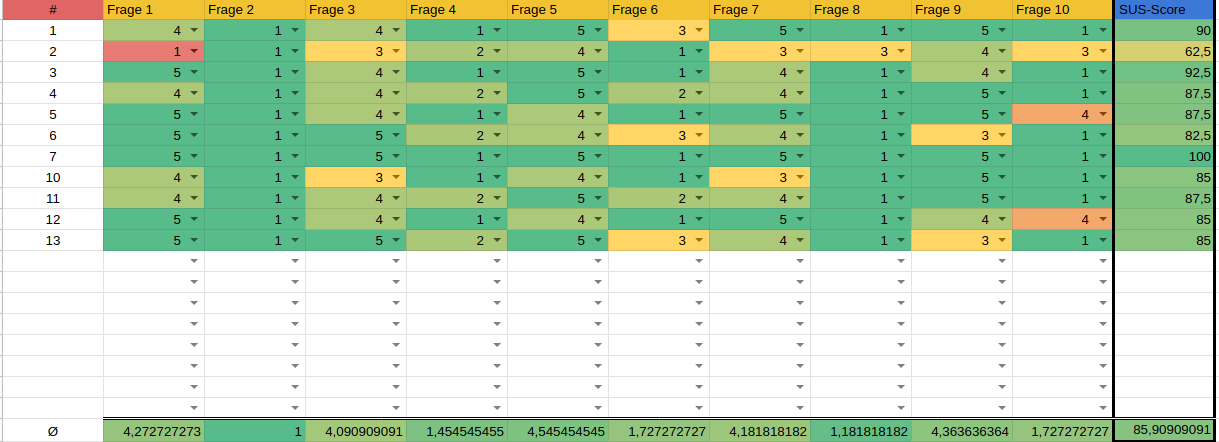
\includegraphics[width=1\linewidth]{figures/SUSscore.png}\par\vspace{1cm}


\subsection{Gelöste Probleme}

\subsubsection{Konfigurationsnamen}
\paragraph{Problem}
Bei der Auswahl der Konfiguration wird nur der interne Name angezeigt (z.B. PolygonConfiguration),
was wenig aussagekräftig ist. Zudem sind diese Namen nicht lokalisiert.

\paragraph{Lösung}
Die IDs der Konfigurationen bekommen einen Eintrag in der Sprachdatei um leicht verständliche
Namen in der gewählen Sprache anzuzeigen.

\subsubsection{Weitere Optimierung der Detailseite für Mobilgeräte}
\paragraph{Symptom}
Auf Mobilgeräten mit besonders kleinen Bildschirmgrößen sind die Diagramme der Detailseite zu klein um Details zu erkennen.

\paragraph{Grund}
Bislang gab es noch kein optimiertes Design dieser Seite für kleine Mobilgeräte.

\paragraph{Lösung}
Die Breakpoints des Grid Layouts wurden angepasst, sodass die Diagramm auf Mobilgeräten nun untereinander, anstatt in Zweierreihen angezeigt werden.

\subsubsection{FeautureSelect-Button}
\paragraph{Symptom}
Das FeatureSelect-Button ist für Personen, die die Webanwendung zum ersten Mal benutzen, schwer zu finden.  

\paragraph{Grund}
Das Button ist zu klein, lässt sich schwer vom Hintergrund unterscheiden. Man hat auch keine Information was es macht bis man draufklickt.

\paragraph{Lösung}
Das FeatureSelect-Menü ist bei Laden der Seite geöffnet und somit für Benutzer leicht zu finden.

\subsubsection{Skala}
\paragraph{Symptom}
Größter Wert der Skala ist unrealistisch groß und damit ist die ganze Skala nutzlos.

\paragraph{Grund}
Skala ist auf den extremen Messwerten aller Messstation festgelegt. 
Da eine Messstation falsche Werte sendet, wird der Skala falsch eingestellt. 

\paragraph{Lösung}
Entsprechende Station aus den Anfragen entfernen.

\subsubsection{Suche}
\paragraph{Symptom}
Der Platzhaltersatz bei der Suche ist nicht vollständig lesbar.

\paragraph{Grund}
Feld  ist zu kurz.

\paragraph{Lösung}
Kürzerer Platzhaltertext. Die Größe des Feldes ist für normaler Städtenamen mehr als ausreichend.

\subsubsection{Vergleich mit letztem Jahr}
\paragraph{Symptom}

Diagramm enthält überhaupt keine Information, was es zeigen will. Der Nutzer kann das Diagramm ohne Erklärung der Entwickler nicht verstehen.


\paragraph{Grund}
Überschrift und Beschriftung der Achsen fehlen.

\paragraph{Lösung}
Überschrift für Diagramme hinzugefügt.

\subsubsection{Polygon}
\paragraph{Symptom}

Man sieht zwar die Färbung der Polygonen, aber man kann ihnen keinen Wert zuordnen.


\paragraph{Grund}
Durchschnittswert der Polygonen wird nirgendwo angezeigt.

\paragraph{Lösung}
Der Durchschnittswert wird in einem Tooltip angezeigt. Dafür musste die Polygonklasse geringfügig
angepasst werden. Sie verwendet nun Observations statt Stations, was eine sinnvolle Erweiterung für die Zukunft ist.


\subsubsection{Namen der Stationen}
\paragraph{Symptom}

Namen und Koordinaten der Stationen sind für die Meisten uninteressant und nichtssagend.
 

\paragraph{Lösung}
Zusätzlich zu den Koordinaten und dem Stationnamen haben wurde auch noch die Straße hinzugefügt.

\subsubsection{Fragezeichen nur auf in der Kartenansicht}
\paragraph{Symptom}
Bei den Stationen-PopUps gibt es ein Fragezeichen-Button, die auf eine Webseite mit mehr Informationen über die ausgewählten Features weiterführt. Es wäre praktisch, diesr Fragezeichen auch auf der detailseite zu haben, insbesondere weil dort alle Features nebeneinander stehen und so man sich alle nacheinender anschauen kann.

\paragraph{Lösung}
Fragezeichen-Button mit gleicher Funktion zu jedem angezeigten Feature auf der Detailseite wurde hinzugefügt.

\subsubsection{Weitere Informationen - Größe und Stelle der Fragezeichen}

\paragraph{Symptom}
Einige Testsubjekte fanden das Fragezeichen einfach zu übersehen und dessen Stelle unpraktisch. Nach mehr Testdurchläufen mit neuen Testsubjekten haben wir festgestellt, dass nur ein kleiner Teil der Testsubjekten das Fragezeichen problematisch gefunden hat. Einige wurden sogar extra von uns darauf angesprochen, ihre Meinung zum Fragezeichen-Button uns mitzuteilen. Sie hatten entweder keine Meinung dazu oder fanden es sogar gut.

\paragraph{Lösung}
Wir haben eine Anleitung zur Webseite hinzugefügt, und deren Button an eine auffällige Stelle platziert. In der Anleitung gibt es auch einen Kapitel über das Fragezeichen-Button mit Illustration. 


\subsection{Unwichtige\textbackslash Unlösbare Probleme}

In diesem Kapitel listen wir die Probleme auf, die wie versucht haben zu lösen, aber die Lösung wäre entweder zu aufwendig gewesen oder hätte nicht in unseren Zeitplan gepasst.


\subsubsection{Sichtbarkeit der Stadtname}
\paragraph{Symptom}
Die Pins bedecken den Stadtnamen. Er ist bei vielen Pins nicht mehr lesbar.

\paragraph{Grund}
Ortbeschriftungen befinden sich auf der Ebene unter den Pins. 

\paragraph{Lösung}
Die Ortsnamen sind direkt in die Kachelbilder eingetragen was es unmöglich macht sie 
auf eine andere Ebene zu verschieben. Eine Option wäre Reverse Geocoding.
